%%%%%%%%%%%%%%%%%%%%%%%%%%%%%%%%%%%%%%%%%%%%%%%%%%%%%%%%%%%%%%%
%
% Welcome to Overleaf --- just edit your LaTeX on the left,
% and we'll compile it for you on the right. If you open the
% 'Share' menu, you can invite other users to edit at the same
% time. See www.overleaf.com/learn for more info. Enjoy!
%
%%%%%%%%%%%%%%%%%%%%%%%%%%%%%%%%%%%%%%%%%%%%%%%%%%%%%%%%%%%%%%%
% Author: Izaak Neutelings (March 2020)
\documentclass[border=3pt,tikz]{standalone}
\usepackage{amsmath} % for \dfrac
\usepackage{physics}
\usepackage{tikz,pgfplots}
\usepackage{tikz-3dplot}
\usepackage[outline]{contour} % glow around text
\usetikzlibrary{angles,quotes} % for pic (angle labels)
\usetikzlibrary{arrows,arrows.meta}
\usetikzlibrary{calc}
\usetikzlibrary{decorations.markings}
\tikzset{>=latex} % for LaTeX arrow head
\usepackage{xcolor}
\colorlet{Ecol}{orange!90!black}
\colorlet{EcolFL}{orange!90!black}
\colorlet{veccol}{green!45!black}
\colorlet{Bcol}{violet!90}
\colorlet{Bcol1}{violet!80!blue!90}
\colorlet{Bcol2}{violet!80!red!90}
\colorlet{BFcol}{red!60!black}
\colorlet{veccol}{green!45!black}
\colorlet{Icol}{blue!70!black}
\tikzstyle{BField}=[->,thick,Bcol]
\tikzstyle{current}=[->,Icol,thick]
\tikzstyle{force}=[->,thick,BFcol]
\tikzstyle{vector}=[->,thick,veccol]
\colorlet{pluscol}{red!60!black}
\colorlet{minuscol}{blue!60!black}
\tikzstyle{charge+}=[very thin,draw=black,top color=red!50,bottom color=red!90!black,shading angle=20,circle,inner sep=0.3]
\tikzstyle{charge-}=[very thin,draw=black,top color=blue!50,bottom color=blue!80,shading angle=20,circle,inner sep=0.3]
\tikzstyle{metal}=[top color=black!15,bottom color=black!25,middle color=black!20,shading angle=10]
\tikzstyle{light metal}=[top color=black!10,bottom color=black!15,middle color=black!6,shading angle=10]
\tikzset{
  EFieldLine/.style={thick,EcolFL,decoration={markings,mark=at position #1 with {\arrow{latex}}},
                     postaction={decorate}},
  EFieldLine/.default=0.5,
  BFieldLine/.style={thick,Bcol,decoration={markings,mark=at position #1 with {\arrow{latex}}},
                                 postaction={decorate}},
  BFieldLine/.default=0.5,
  pics/Bin/.style={
    code={
      \def\R{0.12}
      \draw[pic actions,line width=0.6,#1,fill=white] % ,thick
        (0,0) circle (\R) (-135:.75*\R) -- (45:.75*\R) (-45:.75*\R) -- (135:.75*\R);
  }},
  pics/Bout/.style={
    code={
      \def\R{0.12}
      \draw[pic actions,line width=0.6,#1,fill=white] (0,0) circle (\R);
      \fill[pic actions,#1] (0,0) circle (0.3*\R);
  }},
  pics/Bin/.default=Bcol,
  pics/Bout/.default=Bcol,
  pics/magnet/.style={ %args={#1}
    code={
      \def\h{0.9}
      \coordinate (-N) at (0,\h);
      \coordinate (-S) at (0,-\h);
      \draw[pic actions,thick,top color=red!60,bottom color=red!90,shading angle=20]
        (-0.8*\h/2,0) rectangle ++(0.8*\h,\h);
      \draw[pic actions,thick,top color=blue!60,bottom color=blue!90,shading angle=20]
        (-0.8*\h/2,0) rectangle ++(0.8*\h,-\h);
      \node[pic actions] at (0, \h/2) {\textbf{N}};
      \node[pic actions] at (0,-\h/2) {\textbf{S}};
  }},
}
\tikzstyle{measure}=[<->,fill=white,midway,outer sep=0]
\contourlength{1.5pt}


\begin{document}


% FLUX-CHANGING LOOP
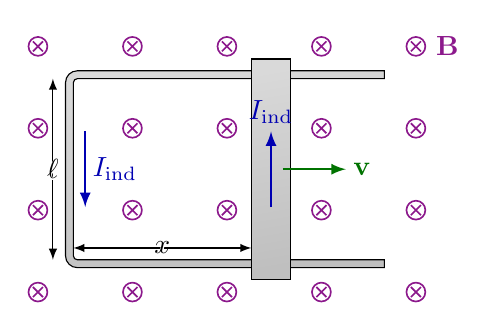
\begin{tikzpicture}
  \def\NBx{5}
  \def\NBy{4}
  \def\L{4.0}
  \def\W{2.4}
  \def\d{4.0}
  \def\t{0.1}
  \def\s{0.64}
  
  % MAGNETIC FIELDLINES
  \foreach \i [evaluate={\y=-0.15*\W+(\i-1)*1.3*\W/(\NBy-1)}] in {1,...,\NBy}{
    \foreach \j [evaluate={\x=-0.1*\L+(\j-1)*1.2*\L/(\NBx-1)}] in {1,...,\NBx}{
      \pic[scale=1] at (\x,\y) {Bin};
    }
  }
  \node[Bcol] at (1.2*\L,1.15*\W) {$\vb{B}$};
  
  % WIRE
  \draw[metal] (\L,\t/2) -- (\t,\t/2) arc (-90:-180:\t/2) -- (\t/2,\W-\t) arc (180:90:\t/2)
                         -- (\L,\W-\t/2) -- (\L,\W+\t/2) -- (\t,\W+\t/2) arc (90:180:1.5*\t)
                         -- (-\t/2,\t) arc (-180:-90:1.5*\t) -- (\L,-\t/2) -- cycle;
  \draw[metal] (\s*\L-2.5*\t,-2*\t) rectangle++ (5*\t,\W+4*\t);
  \draw[vector] (\s*\L+1.5*\t,\W/2) --++ (0.2*\L,0) node[right=-1] {$\vb{v}$};
  \draw[current] (\s*\L,0.3*\W) --++ (0,0.4*\W) node[above=-1] {$I_\text{ind}$};
  \draw[current] (2*\t,0.7*\W) --++ (0,-0.4*\W) node[midway,right=-1] {$I_\text{ind}$};
  \draw[<->] (\t/2,2*\t) -- (\s*\L-2.5*\t,2*\t) node[midway] {\contour{white}{$x$}};
  \draw[<->] (-2.1*\t,\t/2) -- (-2.1*\t,\W-\t/2) node[midway] {\contour{white}{$\ell$}};
  
\end{tikzpicture}


% MOVING CONDUCTOR
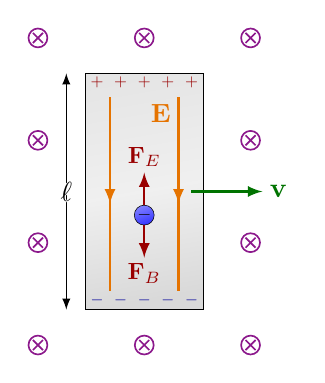
\begin{tikzpicture}
  \def\NBx{3}
  \def\NBy{4}
  \def\NQ{5}
  \def\L{3.0}
  \def\W{1.5}
  
  % MAGNETIC FIELDLINES
  \foreach \i [evaluate={\y=-0.15*\L+(\i-1)*1.3*\L/(\NBy-1)}] in {1,...,\NBy}{
    \foreach \i [evaluate={\x=-0.9*\W+(\i-1)*1.8*\W/(\NBx-1)}] in {1,...,\NBx}{
      \pic[scale=1] at (\x,\y) {Bin};
    }
  }
  
  % CONDUCTOR
  \draw[light metal] (-\W/2,0) rectangle++ (\W,\L);
  \draw[vector] (0.4*\W,\L/2) --++ (0.6*\W,0) node[right=-1] {$\vb{v}$};
  %\draw[current] (\s*\L,0.3*\W) --++ (0,0.4*\W) node[above=-1] {$I_\text{ind}$};
  %\draw[<->] (\t/2,2*\t) -- (\s*\L-2.5*\t,2*\t) node[midway] {\contour{white}{$x$}};
  %\draw[<->] (-2.1*\t,\t/2) -- (-2.1*\t,\W-\t/2) node[midway] {\contour{white}{$h$}};
  \node[charge-,scale=0.65] (Q) at (0,0.40*\L) {$-$};
  \draw[force] (Q) --++ (0, 0.18*\L) node[above=-1,scale=0.85] {$\vb{F}_E$};
  \draw[force] (Q) --++ (0,-0.18*\L) node[below=-1,scale=0.85] {$\vb{F}_B$};
  \draw[<->] (-0.66*\W,0) --++ (0,\L) node[midway] {\contour{white}{$\ell$}};
  \node[Ecol,scale=0.95] at (0.14*\W,0.83*\L) {$\vb{E}$};
  
  % CHARGES
  \foreach \i [evaluate={\x=-\W/2+(\i-0.5)*\W/\NQ}] in {1,...,\NQ}{
    \node[minuscol,scale=0.6] at (\x,0.04*\L) {$-$};
    \node[pluscol,scale=0.6] at (\x,0.96*\L) {$+$};
  }
  \draw[EFieldLine=0.55] (-0.29*\W,0.9*\L) --++ (0,-0.82*\L);
  \draw[EFieldLine=0.55] ( 0.29*\W,0.9*\L) --++ (0,-0.82*\L);
  
\end{tikzpicture}


% MOVING CONDUCTOR
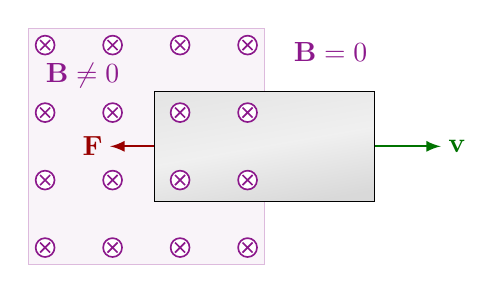
\begin{tikzpicture}
  \def\NBx{4}
  \def\NBy{4}
  \def\WB{3}
  \def\NQ{5}
  \def\L{2.8}
  \def\W{1.4}
  
  % MAGNETIC FIELDLINES
  \draw[Bcol!30,fill=Bcol!5] (-\WB,-\WB/2) rectangle++ (\WB,\WB);
  
  % CONDUCTOR
  \draw[light metal] (-\L/2,-\W/2) rectangle++ (\L,\W);
  \draw[vector] (\W,0) --++ (0.6*\W,0) node[right=-1] {$\vb{v}$};
  \draw[force] (-\W,0) --++ (-0.4*\W,0) node[left=-1] {$\vb{F}$};
  %\draw[EFieldLine=0.55] ( 0.29*\W,0.9*\L) --++ (0,-0.8*\L);
  
  % MAGNETIC FIELDLINES
  \foreach \i [evaluate={\y=-\WB/2+(\i-0.75)*\WB/(\NBy-0.5)}] in {1,...,\NBy}{
    \foreach \j [evaluate={\x=-\WB+(\j-0.75)*\WB/(\NBx-0.5)}] in {1,...,\NBx}{
      \pic[scale=1] at (\x,\y) {Bin};
    }
  }
  \node[Bcol] at (-0.77*\WB,0.30*\WB) {$\vb{B}\neq0$};
  \node[Bcol] at ( 0.28*\WB,0.40*\WB) {$\vb{B}=0$};
  
\end{tikzpicture}


% MAGNET FIELD through current loop - NS in
\def\Rx{0.7}
\def\Ry{1.14}
\def\h{0.5}
\def\H{3}
\def\W{4}
\def\NB{2}
\begin{tikzpicture}
  
  % MAGNETIC FIELD bar magnet
  \draw (0,\Ry) arc (90:270:{\Rx} and {\Ry});
  \foreach \i [evaluate={\x=(0.3-0.1*\i)*\W; \y=(0.35*\H)*\i^2/\NB; \in=180+12*\i^2; \out=1*\i^2; \f=0.4+0.02*\i;}] in {1,...,\NB}{
    \draw[BFieldLine=\f,Bcol1] (-1*\H, 0.45*\y/\H) to[out= \out,in= \in,looseness=0.8] (\x, \y);
    \draw[BFieldLine=\f,Bcol1] (-1*\H,-0.45*\y/\H) to[out=-\out,in=-\in,looseness=0.8] (\x,-\y);
  }
  \pic[rotate=-90] (M) at (-0.95*\W,0) {magnet};
  \node[Bcol1] at (0.15*\W,0.58*\H) {$\vb{B}$};
  \draw[vector] (-0.74*\W,0) --++ (0.2*\W,0) node[right,scale=0.8] {$\vb{v}$};
  
  % INDUCED MAGNETIC FIELD
  \foreach \i [evaluate={\x=(2.0-0.5*\i)*\Rx; \y=\Ry*(\i-0.5)/(\NB-0.25); \in=-10*\i^2; \out=180-\in; \f=0.57;}] in {1,...,\NB}{
    \draw[BFieldLine=\f,Bcol2] (\x, \y) to[out= \out,in= \in,looseness=0.8] (-\x, \y);
    \draw[BFieldLine=\f,Bcol2] (\x,-\y) to[out=-\out,in=-\in,looseness=0.8] (-\x,-\y);
  }
  \node[Bcol2] at (1.6*\Rx,-1.0*\Ry) {$\vb{B}_\text{ind}$};
  
  % CIRCUIT
  \draw[white,very thick]
        (0,\Ry) arc (90:-90:{\Rx} and {\Ry});
  \draw (0,\Ry) arc (90:-90:{\Rx} and {\Ry});
  \draw[current]
    (-110:{1.1*\Rx} and {1.1*\Ry}) arc (-110:-55:{1.1*\Rx} and {1.1*\Ry})
    node[midway,below right=-2] {$I_\text{ind}$};
  
\end{tikzpicture}


% MAGNET FIELD through current loop - NS out
\def\Rx{0.7}
\def\Ry{1.14}
\def\h{0.5}
\def\H{3}
\def\W{4}
\def\NB{2}
\begin{tikzpicture}
  
  % MAGNETIC FIELD bar magnet
  \draw (0,\Ry) arc (90:270:{\Rx} and {\Ry});
  \foreach \i [evaluate={\x=(0.3-0.1*\i)*\W; \y=(0.35*\H)*\i^2/\NB; \in=180+12*\i^2; \out=1*\i^2; \f=0.4+0.02*\i;}] in {1,...,\NB}{
    \draw[BFieldLine=\f,Bcol1] (-1*\H, 0.45*\y/\H) to[out= \out,in= \in,looseness=0.8] (\x, \y);
    \draw[BFieldLine=\f,Bcol1] (-1*\H,-0.45*\y/\H) to[out=-\out,in=-\in,looseness=0.8] (\x,-\y);
  }
  \pic[rotate=-90] (M) at (-0.95*\W,0) {magnet};
  \node[Bcol1] at (0.15*\W,0.58*\H) {$\vb{B}$};
  \draw[vector] (-1.16*\W,0) --++ (-0.2*\W,0) node[left,scale=0.8] {$\vb{v}$};
  
  % INDUCED MAGNETIC FIELD
  \foreach \i [evaluate={\x=(2.0-0.5*\i)*\Rx; \y=\Ry*(\i-0.5)/(\NB-0.25); \in=-10*\i^2; \out=180-\in; \f=0.57;}] in {1,...,\NB}{
    \draw[BFieldLine=\f,Bcol2] (-\x, \y) to[out= \in,in= \out,looseness=0.8] (\x, \y);
    \draw[BFieldLine=\f,Bcol2] (-\x,-\y) to[out=-\in,in=-\out,looseness=0.8] (\x,-\y);
  }
  \node[Bcol2] at (1.6*\Rx,-1.0*\Ry) {$\vb{B}_\text{ind}$};
  
  % CIRCUIT
  \draw[white,very thick]
        (0,\Ry) arc (90:-90:{\Rx} and {\Ry});
  \draw (0,\Ry) arc (90:-90:{\Rx} and {\Ry});
  \draw[current]
    (-60:{1.1*\Rx} and {1.1*\Ry}) arc (-60:-120:{1.1*\Rx} and {1.1*\Ry})
    node[midway,below right=-2] {$I_\text{ind}$};
  
\end{tikzpicture}





% LOOP ENTERING B FIELD
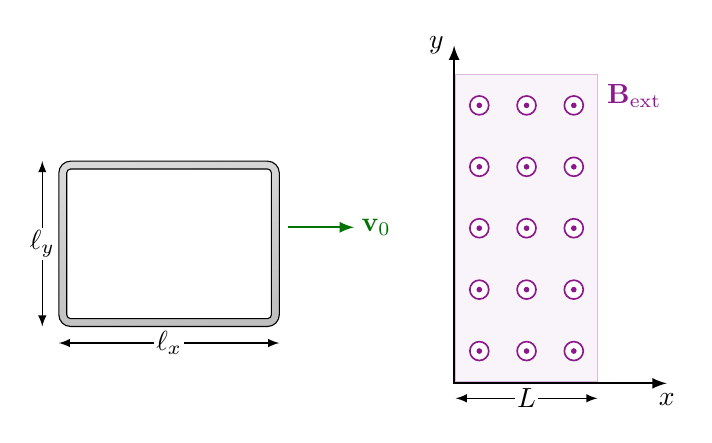
\begin{tikzpicture}
  \def\NBx{3}  % number of B field columns
  \def\NBy{5}  % number of B field rows
  \def\Lx{1.8} % B field width
  \def\Ly{3.9} % B field height
  \def\lx{2.8} % loop width
  \def\ly{2.1} % loop height
  \def\t{0.1}  % loop thickness
  
  % LOOP
  \begin{scope}[shift={(-1.8*\lx,0.18*\Ly)}]
    \draw[metal,rounded corners=1.5*\t cm,even odd rule]
      (0,0) rectangle (\lx,\ly)
      {[rounded corners=0.5*\t cm] (\t,\t) rectangle (\lx-\t,\ly-\t)};
    \draw[vector] (\lx+1.1*\t,0.6*\ly) --++ (0.3*\lx,0) node[right=-1] {$\vb{v}_0$};
    \draw[<->] (0,-2.1*\t) --++ (\lx,0) node[midway,fill=white,inner sep=0.8] {$\ell_x$}; %{\contour{white}{$\ell_x$}};
    \draw[<->] (-2.1*\t,0) --++ (0,\ly) node[midway,fill=white,inner sep=0.8] {$\ell_y$}; %{\contour{white}{$\ell_y$}};
  \end{scope}
  
  % MAGNETIC FIELDLINES
  \draw[Bcol!30,fill=Bcol!5] (0,0) rectangle (\Lx,\Ly);
  \foreach \i [evaluate={\y=(\i-0.5)*\Ly/\NBy}] in {1,...,\NBy}{
    \foreach \j [evaluate={\x=(\j-0.5)*\Lx/\NBx}] in {1,...,\NBx}{
      \pic[scale=1] at (\x,\y) {Bout};
    }
  }
  \node[Bcol,below right] at (\Lx,\Ly) {$\vb{B}_\text{ext}$};
  
  % AXES
  \draw[<->,thick,shift={(-0.02,-0.02)}]
    (0,1.1*\Ly) node[left] {$y$} -- (0,0) -- (1.5*\Lx,0) node[below] {$x$};
  \draw[<->] (0,-2.1*\t) --++ (\Lx,0) node[midway,fill=white,inner sep=0.8] {$L$};
  
\end{tikzpicture}




\end{document}